\documentclass[11pt, a4paper]{article}
\usepackage{apacite}
\usepackage{natbib}
\usepackage[utf8x]{inputenc}
\usepackage[T1]{fontenc}
\usepackage[icelandic]{babel}
\usepackage{amsmath, amsthm, amssymb, amsfonts}
\usepackage{graphicx}
\usepackage{tikz}
\usepackage{tkz-euclide}
\usetkzobj{all}
\usepackage{hyperref}
\usepackage{pgfplots}
\usepackage{geometry}
\usepackage{setspace} 
\usepackage{pdflscape}
\usepackage{mathtools}
\usepackage{fixltx2e}
\usepackage{array}
\setlength\parindent{0pt}
\newtheorem*{problem}{\emph{Problem}}
\newtheorem*{solution}{\emph{Solution}}
\newcommand*\rfrac[2]{{}^{#1}\!/_{#2}} %small fraction
\begin{document}
\begin{titlepage}
\begin{center}

\textsc{\huge Haust 2016}\\[1.5cm]

\textsc{\huge Þýðendur}\\[0.2cm]
\textsc{\huge T-603-THYD}\\[1.5cm]

\end{center}
{ \huge Homework 1\\[1.5cm] }
% Author and supervisor
\Large {
\emph{Nemandi:}\\
Steinn Elliði Pétursson\\[0.5cm]
\emph{Kennitala:}\\
250594-2759\\[0.5cm]
{\large \today}\\[0.5cm]
\emph{Kennari:} \\
Friðjón Guðjohnsen}\\

\end{titlepage}
\leavevmode

\section{}
	Write Regular expressions describing the following languages over the alphabet $\Sigma = {a, b}$
	\subsection*{a)}
			All non-empty strings that start and end with the same symbol.
		\begin{solution}
			$$(a[ab]^{*}a)|(b[ab]^{*}b)|a|b$$
		\end{solution}
	\subsection*{b)}
			All strings that do not have \textit{bbb} as substring ($\epsilon$ included)
		\begin{solution}
			$$^\wedge((?!bbb)[ab])^*\$$$
		\end{solution}
	\subsection*{c)}
		All strings of even length that have aa as a substring.
		\begin{solution}
			$$(ab|ba|bb|aa)^*(aa)^+(ab|ba|bb|aa)^*$$
		\end{solution}
	\subsection*{d)}
		\begin{problem}
		All strings that contain at least one a and at least one b.
		\end{problem}
		\begin{solution}
			$$[ab]^{*}(ab|ba)[ab]^*$$
		\end{solution}
\section{}	
	Use Algorithm 3.23 in the textbook (on page 159) to transform the regular expression $a((aa)^{∗}|b)^∗b$ into a nondeterministic finite automation (NFA). Draw the NFA and show all the intermediate steps in your construction.
	\begin{solution}
		Following are the steps taken to generate an NFA from the above regular expression.
	\end{solution}
	\subsection{}
	a
		\begin{center}
			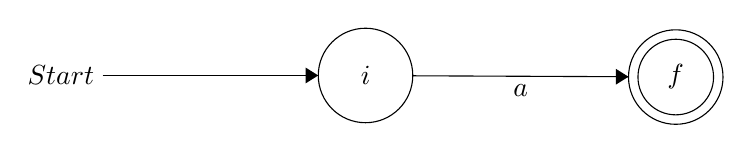
\begin{tikzpicture}[scale=0.2]
			\tikzstyle{every node}+=[inner sep=0pt]
			\draw [black] (25.6,-15.9) circle (3);
			\draw (25.6,-15.9) node {$i$};
			\draw [black] (45.3,-16) circle (3);
			\draw (45.3,-16) node {$f$};
			\draw [black] (45.3,-16) circle (2.4);
			\draw [black] (8.9,-15.9) -- (22.6,-15.9);
			\draw (8.4,-15.9) node [left] {$Start$};
			\fill [black] (22.6,-15.9) -- (21.8,-15.4) -- (21.8,-16.4);
			\draw [black] (28.6,-15.92) -- (42.3,-15.98);
			\fill [black] (42.3,-15.98) -- (41.5,-15.48) -- (41.5,-16.48);
			\draw (35.45,-16.45) node [below] {$a$};
			\end{tikzpicture}
		\end{center}

	\subsection{}
	b
\begin{center}
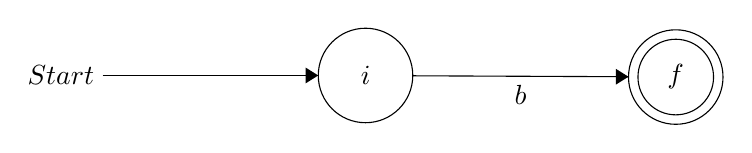
\begin{tikzpicture}[scale=0.2]
\tikzstyle{every node}+=[inner sep=0pt]
\draw [black] (25.6,-15.9) circle (3);
\draw (25.6,-15.9) node {$i$};
\draw [black] (45.3,-16) circle (3);
\draw (45.3,-16) node {$f$};
\draw [black] (45.3,-16) circle (2.4);
\draw [black] (8.9,-15.9) -- (22.6,-15.9);
\draw (8.4,-15.9) node [left] {$Start$};
\fill [black] (22.6,-15.9) -- (21.8,-15.4) -- (21.8,-16.4);
\draw [black] (28.6,-15.92) -- (42.3,-15.98);
\fill [black] (42.3,-15.98) -- (41.5,-15.48) -- (41.5,-16.48);
\draw (35.45,-16.46) node [below] {$b$};
\end{tikzpicture}
\end{center}

	\subsection{}
	aa
		\begin{center}
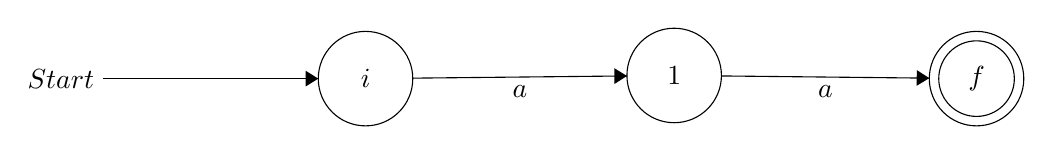
\begin{tikzpicture}[scale=0.2]
\tikzstyle{every node}+=[inner sep=0pt]
\draw [black] (25.7,-16.2) circle (3);
\draw (25.7,-16.2) node {$i$};
\draw [black] (45.3,-16) circle (3);
\draw (45.3,-16) node {$1$};
\draw [black] (64.5,-16.2) circle (3);
\draw (64.5,-16.2) node {$f$};
\draw [black] (64.5,-16.2) circle (2.4);
\draw [black] (9,-16.2) -- (22.7,-16.2);
\draw (8.5,-16.2) node [left] {$Start$};
\fill [black] (22.7,-16.2) -- (21.9,-15.7) -- (21.9,-16.7);
\draw [black] (28.7,-16.17) -- (42.3,-16.03);
\fill [black] (42.3,-16.03) -- (41.5,-15.54) -- (41.51,-16.54);
\draw (35.5,-16.61) node [below] {$a$};
\draw [black] (48.3,-16.03) -- (61.5,-16.17);
\fill [black] (61.5,-16.17) -- (60.71,-15.66) -- (60.69,-16.66);
\draw (54.9,-16.61) node [below] {$a$};
\end{tikzpicture}
\end{center}

	\subsection{}
	$(aa)^*$
		\begin{center}
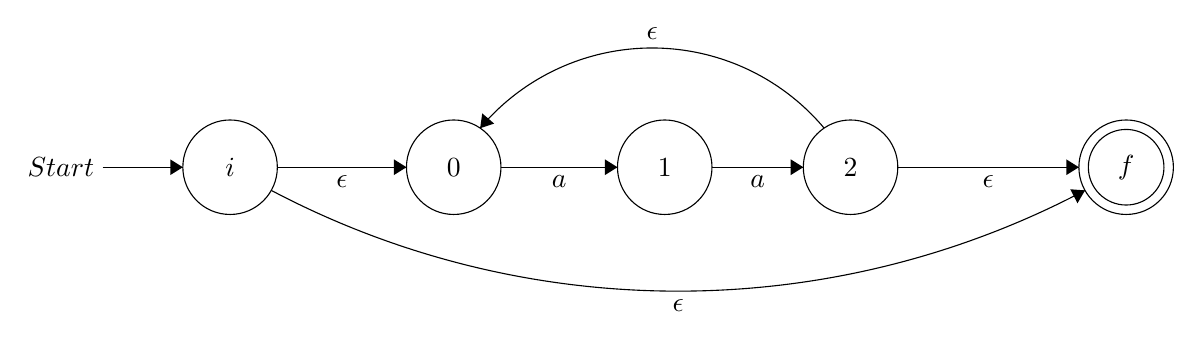
\begin{tikzpicture}[scale=0.2]
\tikzstyle{every node}+=[inner sep=0pt]
\draw [black] (13.8,-16.2) circle (3);
\draw (13.8,-16.2) node {$i$};
\draw [black] (41.4,-16.2) circle (3);
\draw (41.4,-16.2) node {$1$};
\draw [black] (70.7,-16.2) circle (3);
\draw (70.7,-16.2) node {$f$};
\draw [black] (70.7,-16.2) circle (2.4);
\draw [black] (28,-16.2) circle (3);
\draw (28,-16.2) node {$0$};
\draw [black] (53.2,-16.2) circle (3);
\draw (53.2,-16.2) node {$2$};
\draw [black] (5.7,-16.2) -- (10.8,-16.2);
\draw (5.2,-16.2) node [left] {$Start$};
\fill [black] (10.8,-16.2) -- (10,-15.7) -- (10,-16.7);
\draw [black] (16.8,-16.2) -- (25,-16.2);
\fill [black] (25,-16.2) -- (24.2,-15.7) -- (24.2,-16.7);
\draw (20.9,-16.7) node [below] {$\epsilon$};
\draw [black] (31,-16.2) -- (38.4,-16.2);
\fill [black] (38.4,-16.2) -- (37.6,-15.7) -- (37.6,-16.7);
\draw (34.7,-16.7) node [below] {$a$};
\draw [black] (44.4,-16.2) -- (50.2,-16.2);
\fill [black] (50.2,-16.2) -- (49.4,-15.7) -- (49.4,-16.7);
\draw (47.3,-16.7) node [below] {$a$};
\draw [black] (56.2,-16.2) -- (67.7,-16.2);
\fill [black] (67.7,-16.2) -- (66.9,-15.7) -- (66.9,-16.7);
\draw (61.95,-16.7) node [below] {$\epsilon$};
\draw [black] (29.675,-13.718) arc (139.9625:40.0375:14.269);
\fill [black] (29.68,-13.72) -- (30.57,-13.43) -- (29.81,-12.78);
\draw (40.6,-8.13) node [above] {$\epsilon$};
\draw [black] (68.086,-17.671) arc (-62.17531:-117.82469:55.351);
\fill [black] (68.09,-17.67) -- (67.15,-17.6) -- (67.61,-18.49);
\draw (42.25,-24.57) node [below] {$\epsilon$};
\end{tikzpicture}
\end{center}

	\subsection{}
	$(aa)^{*}|b$
	\begin{center}
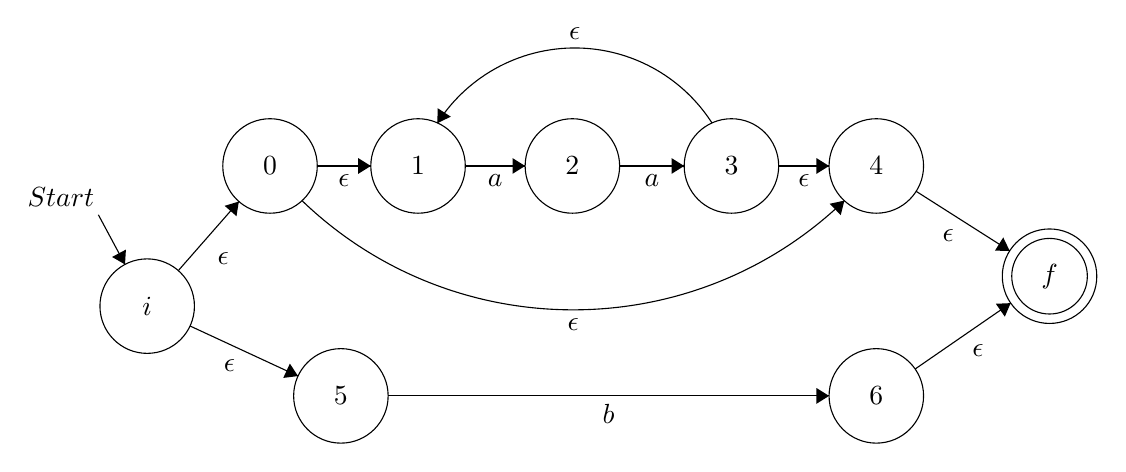
\begin{tikzpicture}[scale=0.2]
\tikzstyle{every node}+=[inner sep=0pt]
\draw [black] (16.5,-17.5) circle (3);
\draw (16.5,-17.5) node {$0$};
\draw [black] (35.7,-17.5) circle (3);
\draw (35.7,-17.5) node {$2$};
\draw [black] (55,-17.5) circle (3);
\draw (55,-17.5) node {$4$};
\draw [black] (25.9,-17.5) circle (3);
\draw (25.9,-17.5) node {$1$};
\draw [black] (45.8,-17.5) circle (3);
\draw (45.8,-17.5) node {$3$};
\draw [black] (8.7,-26.4) circle (3);
\draw (8.7,-26.4) node {$i$};
\draw [black] (21,-32.1) circle (3);
\draw (21,-32.1) node {$5$};
\draw [black] (55,-32.1) circle (3);
\draw (55,-32.1) node {$6$};
\draw [black] (66,-24.5) circle (3);
\draw (66,-24.5) node {$f$};
\draw [black] (66,-24.5) circle (2.4);
\draw [black] (19.5,-17.5) -- (22.9,-17.5);
\fill [black] (22.9,-17.5) -- (22.1,-17) -- (22.1,-18);
\draw (21.2,-18) node [below] {$\epsilon$};
\draw [black] (28.9,-17.5) -- (32.7,-17.5);
\fill [black] (32.7,-17.5) -- (31.9,-17) -- (31.9,-18);
\draw (30.8,-18) node [below] {$a$};
\draw [black] (38.7,-17.5) -- (42.8,-17.5);
\fill [black] (42.8,-17.5) -- (42,-17) -- (42,-18);
\draw (40.75,-18) node [below] {$a$};
\draw [black] (48.8,-17.5) -- (52,-17.5);
\fill [black] (52,-17.5) -- (51.2,-17) -- (51.2,-18);
\draw (50.4,-18) node [below] {$\epsilon$};
\draw [black] (27.132,-14.776) arc (147.36578:32.63422:10.353);
\fill [black] (27.13,-14.78) -- (27.98,-14.37) -- (27.14,-13.83);
\draw (35.85,-9.51) node [above] {$\epsilon$};
\draw [black] (52.968,-19.704) arc (-46.13364:-133.86636:24.846);
\fill [black] (52.97,-19.7) -- (52.04,-19.9) -- (52.74,-20.62);
\draw (35.75,-27.14) node [below] {$\epsilon$};
\draw [black] (5.6,-20.6) -- (7.29,-23.75);
\draw (3.22,-20.09) node [above] {$Start$};
\fill [black] (7.29,-23.75) -- (7.35,-22.81) -- (6.47,-23.28);
\draw [black] (10.68,-24.14) -- (14.52,-19.76);
\fill [black] (14.52,-19.76) -- (13.62,-20.03) -- (14.37,-20.69);
\draw (13.14,-23.4) node [right] {$\epsilon$};
\draw [black] (24,-32.1) -- (52,-32.1);
\fill [black] (52,-32.1) -- (51.2,-31.6) -- (51.2,-32.6);
\draw (38,-32.6) node [below] {$b$};
\draw [black] (11.42,-27.66) -- (18.28,-30.84);
\fill [black] (18.28,-30.84) -- (17.76,-30.05) -- (17.34,-30.96);
\draw (13.92,-29.76) node [below] {$\epsilon$};
\draw [black] (57.53,-19.11) -- (63.47,-22.89);
\fill [black] (63.47,-22.89) -- (63.06,-22.04) -- (62.53,-22.88);
\draw (59.56,-21.5) node [below] {$\epsilon$};
\draw [black] (57.47,-30.39) -- (63.53,-26.21);
\fill [black] (63.53,-26.21) -- (62.59,-26.25) -- (63.16,-27.07);
\draw (61.45,-28.8) node [below] {$\epsilon$};
\end{tikzpicture}
\end{center}


	\subsection{}
		$((aa)^{*}|b)^*$
		\begin{center}
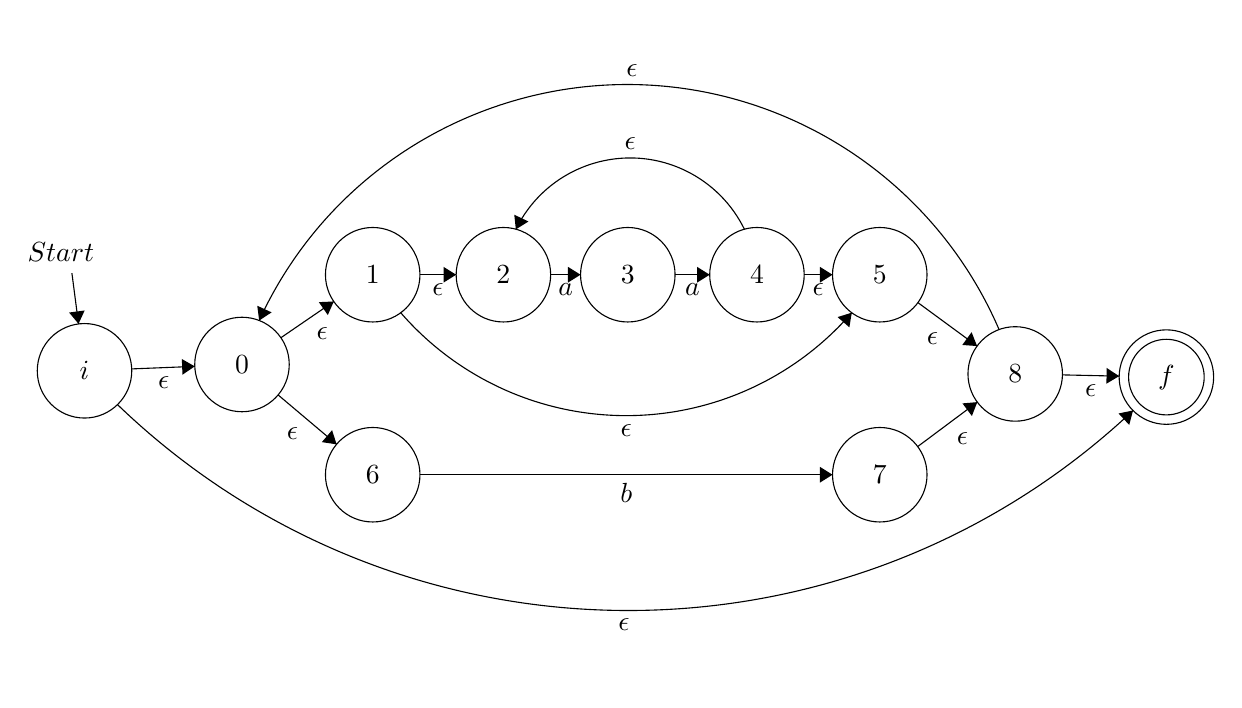
\begin{tikzpicture}[scale=0.2]
\tikzstyle{every node}+=[inner sep=0pt]
\draw [black] (24.1,-17.5) circle (3);
\draw (24.1,-17.5) node {$1$};
\draw [black] (40.3,-17.5) circle (3);
\draw (40.3,-17.5) node {$3$};
\draw [black] (56.3,-17.5) circle (3);
\draw (56.3,-17.5) node {$5$};
\draw [black] (32.4,-17.5) circle (3);
\draw (32.4,-17.5) node {$2$};
\draw [black] (48.5,-17.5) circle (3);
\draw (48.5,-17.5) node {$4$};
\draw [black] (15.8,-23.2) circle (3);
\draw (15.8,-23.2) node {$0$};
\draw [black] (24.1,-30.2) circle (3);
\draw (24.1,-30.2) node {$6$};
\draw [black] (56.3,-30.2) circle (3);
\draw (56.3,-30.2) node {$7$};
\draw [black] (5.8,-23.6) circle (3);
\draw (5.8,-23.6) node {$i$};
\draw [black] (64.9,-23.8) circle (3);
\draw (64.9,-23.8) node {$8$};
\draw [black] (74.5,-24) circle (3);
\draw (74.5,-24) node {$f$};
\draw [black] (74.5,-24) circle (2.4);
\draw [black] (27.1,-17.5) -- (29.4,-17.5);
\fill [black] (29.4,-17.5) -- (28.6,-17) -- (28.6,-18);
\draw (28.25,-18) node [below] {$\epsilon$};
\draw [black] (35.4,-17.5) -- (37.3,-17.5);
\fill [black] (37.3,-17.5) -- (36.5,-17) -- (36.5,-18);
\draw (36.35,-18) node [below] {$a$};
\draw [black] (43.3,-17.5) -- (45.5,-17.5);
\fill [black] (45.5,-17.5) -- (44.7,-17) -- (44.7,-18);
\draw (44.4,-18) node [below] {$a$};
\draw [black] (51.5,-17.5) -- (53.3,-17.5);
\fill [black] (53.3,-17.5) -- (52.5,-17) -- (52.5,-18);
\draw (52.4,-18) node [below] {$\epsilon$};
\draw [black] (33.189,-14.624) arc (154.01639:25.98361:8.077);
\fill [black] (33.19,-14.62) -- (33.99,-14.12) -- (33.09,-13.69);
\draw (40.45,-9.59) node [above] {$\epsilon$};
\draw [black] (54.521,-19.912) arc (-40.94128:-139.05872:18.959);
\fill [black] (54.52,-19.91) -- (53.62,-20.19) -- (54.37,-20.84);
\draw (40.2,-26.95) node [below] {$\epsilon$};
\draw [black] (18.27,-21.5) -- (21.63,-19.2);
\fill [black] (21.63,-19.2) -- (20.68,-19.24) -- (21.25,-20.06);
\draw (20.9,-20.85) node [below] {$\epsilon$};
\draw [black] (27.1,-30.2) -- (53.3,-30.2);
\fill [black] (53.3,-30.2) -- (52.5,-29.7) -- (52.5,-30.7);
\draw (40.2,-30.7) node [below] {$b$};
\draw [black] (18.09,-25.13) -- (21.81,-28.27);
\fill [black] (21.81,-28.27) -- (21.52,-27.37) -- (20.87,-28.13);
\draw (19,-27.19) node [below] {$\epsilon$};
\draw [black] (5,-17.4) -- (5.42,-20.62);
\draw (4.3,-16.68) node [above] {$Start$};
\fill [black] (5.42,-20.62) -- (5.81,-19.77) -- (4.82,-19.9);
\draw [black] (8.8,-23.48) -- (12.8,-23.32);
\fill [black] (12.8,-23.32) -- (11.98,-22.85) -- (12.02,-23.85);
\draw (10.83,-23.94) node [below] {$\epsilon$};
\draw [black] (58.71,-28.41) -- (62.49,-25.59);
\fill [black] (62.49,-25.59) -- (61.55,-25.67) -- (62.15,-26.47);
\draw (61.55,-27.5) node [below] {$\epsilon$};
\draw [black] (58.72,-19.27) -- (62.48,-22.03);
\fill [black] (62.48,-22.03) -- (62.13,-21.15) -- (61.54,-21.96);
\draw (59.65,-21.15) node [below] {$\epsilon$};
\draw [black] (16.89,-20.407) arc (155.3301:23.26967:25.713);
\fill [black] (16.89,-20.41) -- (17.68,-19.89) -- (16.77,-19.47);
\draw (40.57,-4.92) node [above] {$\epsilon$};
\draw [black] (67.9,-23.86) -- (71.5,-23.94);
\fill [black] (71.5,-23.94) -- (70.71,-23.42) -- (70.69,-24.42);
\draw (69.69,-24.42) node [below] {$\epsilon$};
\draw [black] (72.382,-26.124) arc (-46.76405:-133.90314:46.783);
\fill [black] (72.38,-26.12) -- (71.46,-26.31) -- (72.14,-27.04);
\draw (40.06,-39.33) node [below] {$\epsilon$};
\end{tikzpicture}
\end{center}

	\subsection{}
		$a((aa)^{*}|b)^*$
		\begin{center}
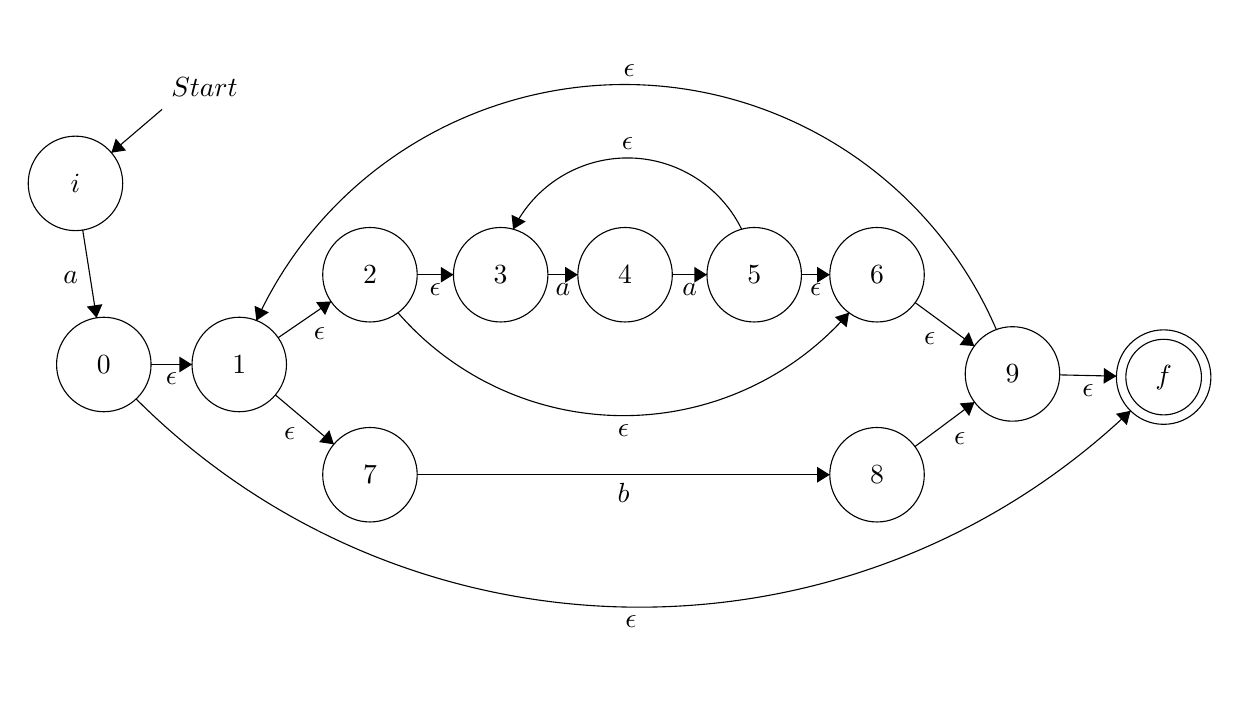
\begin{tikzpicture}[scale=0.2]
\tikzstyle{every node}+=[inner sep=0pt]
\draw [black] (24.1,-17.5) circle (3);
\draw (24.1,-17.5) node {$2$};
\draw [black] (40.3,-17.5) circle (3);
\draw (40.3,-17.5) node {$4$};
\draw [black] (56.3,-17.5) circle (3);
\draw (56.3,-17.5) node {$6$};
\draw [black] (32.4,-17.5) circle (3);
\draw (32.4,-17.5) node {$3$};
\draw [black] (48.5,-17.5) circle (3);
\draw (48.5,-17.5) node {$5$};
\draw [black] (15.8,-23.2) circle (3);
\draw (15.8,-23.2) node {$1$};
\draw [black] (24.1,-30.2) circle (3);
\draw (24.1,-30.2) node {$7$};
\draw [black] (56.3,-30.2) circle (3);
\draw (56.3,-30.2) node {$8$};
\draw [black] (7.2,-23.2) circle (3);
\draw (7.2,-23.2) node {$0$};
\draw [black] (64.9,-23.8) circle (3);
\draw (64.9,-23.8) node {$9$};
\draw [black] (74.5,-24) circle (3);
\draw (74.5,-24) node {$f$};
\draw [black] (74.5,-24) circle (2.4);
\draw [black] (5.4,-11.7) circle (3);
\draw (5.4,-11.7) node {$i$};
\draw [black] (27.1,-17.5) -- (29.4,-17.5);
\fill [black] (29.4,-17.5) -- (28.6,-17) -- (28.6,-18);
\draw (28.25,-18) node [below] {$\epsilon$};
\draw [black] (35.4,-17.5) -- (37.3,-17.5);
\fill [black] (37.3,-17.5) -- (36.5,-17) -- (36.5,-18);
\draw (36.35,-18) node [below] {$a$};
\draw [black] (43.3,-17.5) -- (45.5,-17.5);
\fill [black] (45.5,-17.5) -- (44.7,-17) -- (44.7,-18);
\draw (44.4,-18) node [below] {$a$};
\draw [black] (51.5,-17.5) -- (53.3,-17.5);
\fill [black] (53.3,-17.5) -- (52.5,-17) -- (52.5,-18);
\draw (52.4,-18) node [below] {$\epsilon$};
\draw [black] (33.189,-14.624) arc (154.01639:25.98361:8.077);
\fill [black] (33.19,-14.62) -- (33.99,-14.12) -- (33.09,-13.69);
\draw (40.45,-9.59) node [above] {$\epsilon$};
\draw [black] (54.521,-19.912) arc (-40.94128:-139.05872:18.959);
\fill [black] (54.52,-19.91) -- (53.62,-20.19) -- (54.37,-20.84);
\draw (40.2,-26.95) node [below] {$\epsilon$};
\draw [black] (18.27,-21.5) -- (21.63,-19.2);
\fill [black] (21.63,-19.2) -- (20.68,-19.24) -- (21.25,-20.06);
\draw (20.9,-20.85) node [below] {$\epsilon$};
\draw [black] (27.1,-30.2) -- (53.3,-30.2);
\fill [black] (53.3,-30.2) -- (52.5,-29.7) -- (52.5,-30.7);
\draw (40.2,-30.7) node [below] {$b$};
\draw [black] (18.09,-25.13) -- (21.81,-28.27);
\fill [black] (21.81,-28.27) -- (21.52,-27.37) -- (20.87,-28.13);
\draw (19,-27.19) node [below] {$\epsilon$};
\draw [black] (10.2,-23.2) -- (12.8,-23.2);
\fill [black] (12.8,-23.2) -- (12,-22.7) -- (12,-23.7);
\draw (11.5,-23.7) node [below] {$\epsilon$};
\draw [black] (58.71,-28.41) -- (62.49,-25.59);
\fill [black] (62.49,-25.59) -- (61.55,-25.67) -- (62.15,-26.47);
\draw (61.55,-27.5) node [below] {$\epsilon$};
\draw [black] (58.72,-19.27) -- (62.48,-22.03);
\fill [black] (62.48,-22.03) -- (62.13,-21.15) -- (61.54,-21.96);
\draw (59.65,-21.15) node [below] {$\epsilon$};
\draw [black] (16.89,-20.407) arc (155.3301:23.26967:25.713);
\fill [black] (16.89,-20.41) -- (17.68,-19.89) -- (16.77,-19.47);
\draw (40.57,-4.92) node [above] {$\epsilon$};
\draw [black] (67.9,-23.86) -- (71.5,-23.94);
\fill [black] (71.5,-23.94) -- (70.71,-23.42) -- (70.69,-24.42);
\draw (69.69,-24.42) node [below] {$\epsilon$};
\draw [black] (72.397,-26.139) arc (-46.40649:-134.95561:45.231);
\fill [black] (72.4,-26.14) -- (71.47,-26.33) -- (72.16,-27.05);
\draw (40.67,-39.12) node [below] {$\epsilon$};
\draw [black] (10.9,-7) -- (7.68,-9.75);
\draw (11.45,-5.56) node [right] {$Start$};
\fill [black] (7.68,-9.75) -- (8.61,-9.61) -- (7.96,-8.85);
\draw [black] (5.86,-14.66) -- (6.74,-20.24);
\fill [black] (6.74,-20.24) -- (7.11,-19.37) -- (6.12,-19.52);
\draw (5.6,-17.65) node [left] {$a$};
\end{tikzpicture}
\end{center}

	\subsection{}
		$a((aa)^{*}|b)^{*}b$ The fully constructed NFA
		\begin{center}
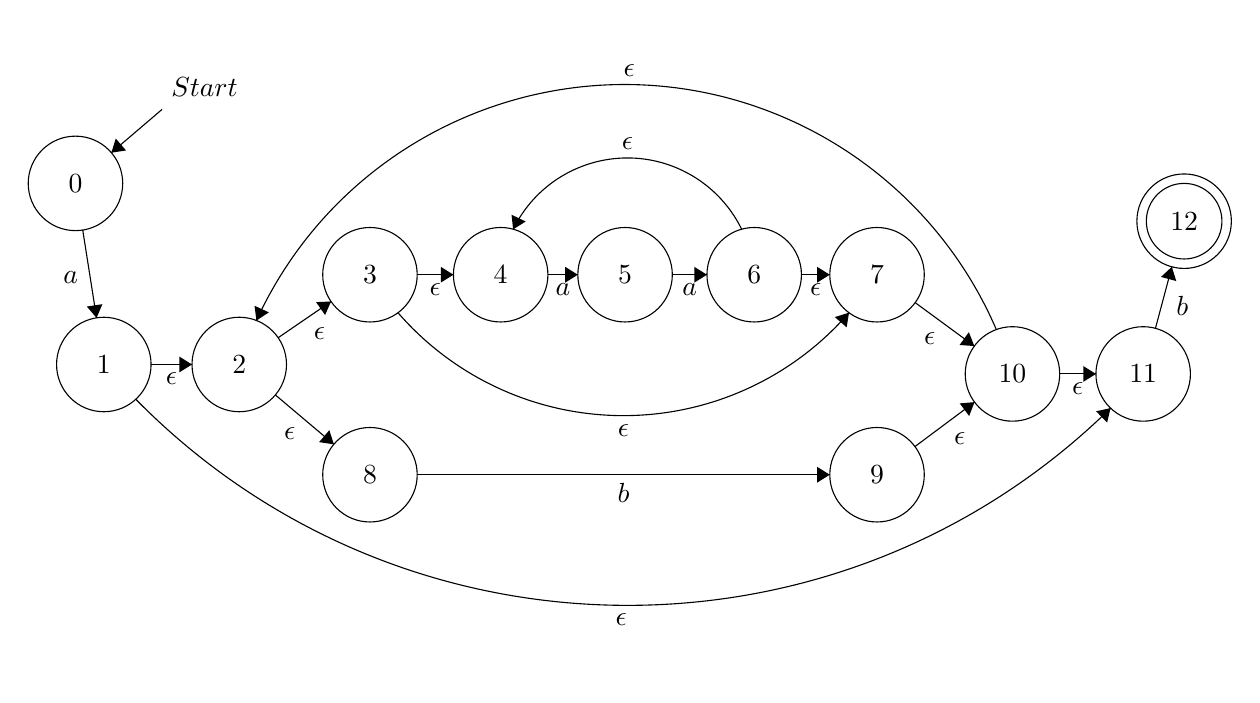
\begin{tikzpicture}[scale=0.2]
\tikzstyle{every node}+=[inner sep=0pt]
\draw [black] (24.1,-17.5) circle (3);
\draw (24.1,-17.5) node {$3$};
\draw [black] (40.3,-17.5) circle (3);
\draw (40.3,-17.5) node {$5$};
\draw [black] (56.3,-17.5) circle (3);
\draw (56.3,-17.5) node {$7$};
\draw [black] (32.4,-17.5) circle (3);
\draw (32.4,-17.5) node {$4$};
\draw [black] (48.5,-17.5) circle (3);
\draw (48.5,-17.5) node {$6$};
\draw [black] (15.8,-23.2) circle (3);
\draw (15.8,-23.2) node {$2$};
\draw [black] (24.1,-30.2) circle (3);
\draw (24.1,-30.2) node {$8$};
\draw [black] (56.3,-30.2) circle (3);
\draw (56.3,-30.2) node {$9$};
\draw [black] (7.2,-23.2) circle (3);
\draw (7.2,-23.2) node {$1$};
\draw [black] (64.9,-23.8) circle (3);
\draw (64.9,-23.8) node {$10$};
\draw [black] (73.2,-23.8) circle (3);
\draw (73.2,-23.8) node {$11$};
\draw [black] (5.4,-11.7) circle (3);
\draw (5.4,-11.7) node {$0$};
\draw [black] (75.8,-14.1) circle (3);
\draw (75.8,-14.1) node {$12$};
\draw [black] (75.8,-14.1) circle (2.4);
\draw [black] (27.1,-17.5) -- (29.4,-17.5);
\fill [black] (29.4,-17.5) -- (28.6,-17) -- (28.6,-18);
\draw (28.25,-18) node [below] {$\epsilon$};
\draw [black] (35.4,-17.5) -- (37.3,-17.5);
\fill [black] (37.3,-17.5) -- (36.5,-17) -- (36.5,-18);
\draw (36.35,-18) node [below] {$a$};
\draw [black] (43.3,-17.5) -- (45.5,-17.5);
\fill [black] (45.5,-17.5) -- (44.7,-17) -- (44.7,-18);
\draw (44.4,-18) node [below] {$a$};
\draw [black] (51.5,-17.5) -- (53.3,-17.5);
\fill [black] (53.3,-17.5) -- (52.5,-17) -- (52.5,-18);
\draw (52.4,-18) node [below] {$\epsilon$};
\draw [black] (33.189,-14.624) arc (154.01639:25.98361:8.077);
\fill [black] (33.19,-14.62) -- (33.99,-14.12) -- (33.09,-13.69);
\draw (40.45,-9.59) node [above] {$\epsilon$};
\draw [black] (54.521,-19.912) arc (-40.94128:-139.05872:18.959);
\fill [black] (54.52,-19.91) -- (53.62,-20.19) -- (54.37,-20.84);
\draw (40.2,-26.95) node [below] {$\epsilon$};
\draw [black] (18.27,-21.5) -- (21.63,-19.2);
\fill [black] (21.63,-19.2) -- (20.68,-19.24) -- (21.25,-20.06);
\draw (20.9,-20.85) node [below] {$\epsilon$};
\draw [black] (27.1,-30.2) -- (53.3,-30.2);
\fill [black] (53.3,-30.2) -- (52.5,-29.7) -- (52.5,-30.7);
\draw (40.2,-30.7) node [below] {$b$};
\draw [black] (18.09,-25.13) -- (21.81,-28.27);
\fill [black] (21.81,-28.27) -- (21.52,-27.37) -- (20.87,-28.13);
\draw (19,-27.19) node [below] {$\epsilon$};
\draw [black] (10.2,-23.2) -- (12.8,-23.2);
\fill [black] (12.8,-23.2) -- (12,-22.7) -- (12,-23.7);
\draw (11.5,-23.7) node [below] {$\epsilon$};
\draw [black] (58.71,-28.41) -- (62.49,-25.59);
\fill [black] (62.49,-25.59) -- (61.55,-25.67) -- (62.15,-26.47);
\draw (61.55,-27.5) node [below] {$\epsilon$};
\draw [black] (58.72,-19.27) -- (62.48,-22.03);
\fill [black] (62.48,-22.03) -- (62.13,-21.15) -- (61.54,-21.96);
\draw (59.65,-21.15) node [below] {$\epsilon$};
\draw [black] (16.89,-20.407) arc (155.3301:23.26967:25.713);
\fill [black] (16.89,-20.41) -- (17.68,-19.89) -- (16.77,-19.47);
\draw (40.57,-4.92) node [above] {$\epsilon$};
\draw [black] (67.9,-23.8) -- (70.2,-23.8);
\fill [black] (70.2,-23.8) -- (69.4,-23.3) -- (69.4,-24.3);
\draw (69.05,-24.3) node [below] {$\epsilon$};
\draw [black] (71.131,-25.972) arc (-45.56961:-135.4721:43.811);
\fill [black] (71.13,-25.97) -- (70.21,-26.17) -- (70.91,-26.89);
\draw (40.06,-39) node [below] {$\epsilon$};
\draw [black] (10.9,-7) -- (7.68,-9.75);
\draw (11.45,-5.56) node [right] {$Start$};
\fill [black] (7.68,-9.75) -- (8.61,-9.61) -- (7.96,-8.85);
\draw [black] (5.86,-14.66) -- (6.74,-20.24);
\fill [black] (6.74,-20.24) -- (7.11,-19.37) -- (6.12,-19.52);
\draw (5.6,-17.65) node [left] {$a$};
\draw [black] (73.98,-20.9) -- (75.02,-17);
\fill [black] (75.02,-17) -- (74.33,-17.64) -- (75.3,-17.9);
\draw (75.27,-19.46) node [right] {$b$};
\end{tikzpicture}
\end{center}

\section{}
	Use algorithm 3.20 in the textbook (on page 153) to transform the NFA you constructed in Exercise 3 into a DFA. Draw the DFA and show all intermediate steps.
	\begin{solution}\end{solution}
		Let's start by finding the start state of the DFA: $\epsilon -closure(0) = A = \{0\}$. \\
		Next let's find the transitions for a and b: \\
		$Dtran[A,a] = \epsilon -closure(move(A,a))$ \\
		$move(A,a) = \{1\}$ \\
		$\epsilon -closure(\{1\}) = \{1,2,3,4,7,8,10,11\}$\\ 
		Let us call this set B\\
		$Dtran[A,b] = \epsilon -closure(move(A,b))$ \\
		$move(A,b) = \{\}$ \\
		$\epsilon -closure(\{\}) = \{\}$\\ 
		This results in an invalid state which shall be called F. The invalid state can only redirect to itself since there is no way to end up with a valid solution if we end up in the invalid state.

		After the above transition we have the following transition table.\\
		\begin{tabular}{|l|l||l|l|}
			\hline
			NFA State & DFA State & a & b \\
			\hline
			\{0\} & A & B & F \\
			\hline
			\{1,2,3,4,7,8,10,11\} & B & ? & ?\\
			\hline
			\{\} & F & F & F \\
			\hline
		\end{tabular}~\\~\\
		Now let us apply the algorithm on set B: \\
		$Dtran[B,a] = \epsilon -closure(move(B,a))$~\\
		$move(B,a) = \{5\}$\\
		$\epsilon -closure(\{5\}) = \{5\}$\\ 
		This gives us $Dtran[B,a] = \{5\}$ let's call this set C\\
		$Dtran[B,b] = \epsilon -closure(move(B,b))$~\\
		$move(B,b) = \{9,12\}$\\
		$\epsilon -closure(\{9,12\}) = \{2,3,4,7,8,9,10,11,12\}$\\ 
		This gives us $Dtran[B,a] = \{2,3,4,7,8,9,10,11,12\}$ let's call this set D. \\
		Now we have the following transition table: \\
		\begin{tabular}{|l|l||l|l|}
			\hline
			NFA State & DFA State & a & b \\
			\hline
			\{0\} & A & B & F \\
			\hline
			\{1,2,3,4,7,8,10,11\} & B & C & D\\
			\hline
			\{5\} & C & ? & ? \\
			\hline
			\{2,3,4,7,8,9,10,11,12\} & D & ? & ? \\
			\hline
			\{\} & F & F & F \\
			\hline
		\end{tabular}~\\~\\
		Let's next apply the algorithm on set C: \\
		$Dtran[C,a] = \epsilon -closure(move(C,a))$~\\
		$move(C,a) = \{6\}$\\
		$\epsilon -closure(\{6\}) = \{2,3,4,6,7,8,10,11\}$\\ 
		This gives us $Dtran[B,a] = \{2,3,4,6,7,8,10,11\}$ let's call this set E\\
		$Dtran[C,b] = \epsilon -closure(move(C,b))$~\\
		$move(C,b) = \{\}$\\
		$\epsilon -closure(\{\}) = \{\}$\\ 
		This results in the invalid state F \\
		Now we have the following transition table: \\
		\begin{tabular}{|l|l||l|l|}
			\hline
			NFA State & DFA State & a & b \\
			\hline
			\{0\} & A & B & F \\
			\hline
			\{1,2,3,4,7,8,10,11\} & B & C & D\\
			\hline
			\{5\} & C & E & F \\
			\hline
			\{2,3,4,7,8,9,10,11,12\} & D & ? & ? \\
			\hline
			\{2,3,4,6,7,8,10,11\} & E & ? & ? \\
			\hline
			\{\} & F & F & F \\
			\hline
		\end{tabular}~\\~\\
		Applying the same methods on sets D and E we get the following results:\\
		$Dtran[D,a] = \{5\}$ which is equal to the set C. \\
		$Dtran[D,b] = \{2,3,4,7,8,9,10,11,12\}$ which is equal to D itself. \\
		$Dtran[E,a] = \{5\}$ which is equal to the set C. \\
		$Dtran[E,b] = \{2,3,4,7,8,9,10,11,12\}$ which is equal to D. \\
		This gives us the complete transition table for the NFA: \\
		\begin{tabular}{|l|l||l|l|}
			\hline
			NFA State & DFA State & a & b \\
			\hline
			\{0\} & A & B & F \\
			\hline
			\{1,2,3,4,7,8,10,11\} & B & C & D\\
			\hline
			\{5\} & C & E & F \\
			\hline
			\{2,3,4,7,8,9,10,11,12\} & D & C & D \\
			\hline
			\{2,3,4,6,7,8,10,11\} & E & C & D \\
			\hline
			\{\} & F & F & F \\
			\hline
		\end{tabular}~\\~\\
		Following is the DFA constructed from the transition table: \\
\begin{center}
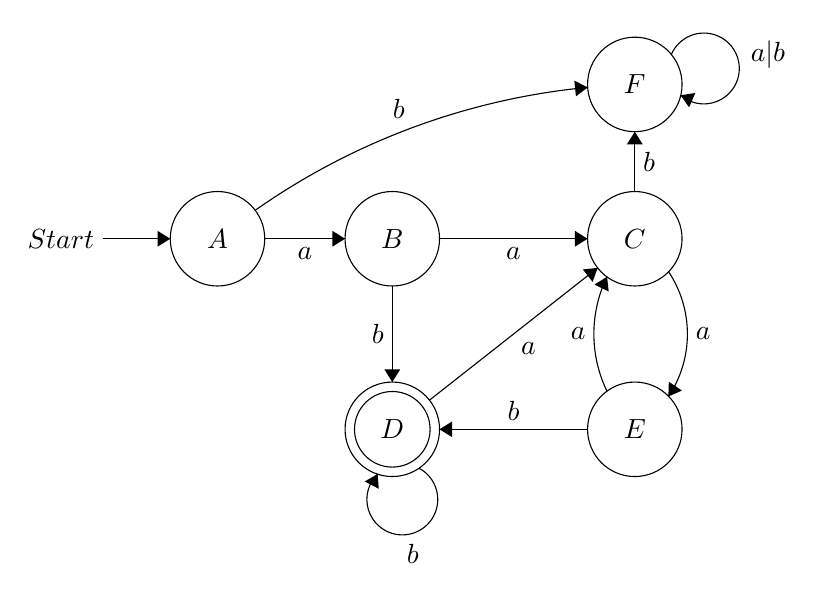
\begin{tikzpicture}[scale=0.2]
\tikzstyle{every node}+=[inner sep=0pt]
\draw [black] (14.1,-16.8) circle (3);
\draw (14.1,-16.8) node {$A$};
\draw [black] (25.2,-16.8) circle (3);
\draw (25.2,-16.8) node {$B$};
\draw [black] (40.6,-16.8) circle (3);
\draw (40.6,-16.8) node {$C$};
\draw [black] (25.2,-28.9) circle (3);
\draw (25.2,-28.9) node {$D$};
\draw [black] (25.2,-28.9) circle (2.4);
\draw [black] (40.6,-28.9) circle (3);
\draw (40.6,-28.9) node {$E$};
\draw [black] (40.6,-7) circle (3);
\draw (40.6,-7) node {$F$};
\draw [black] (6.8,-16.8) -- (11.1,-16.8);
\draw (6.3,-16.8) node [left] {$Start$};
\fill [black] (11.1,-16.8) -- (10.3,-16.3) -- (10.3,-17.3);
\draw [black] (17.1,-16.8) -- (22.2,-16.8);
\fill [black] (22.2,-16.8) -- (21.4,-16.3) -- (21.4,-17.3);
\draw (19.65,-17.3) node [below] {$a$};
\draw [black] (25.2,-19.8) -- (25.2,-25.9);
\fill [black] (25.2,-25.9) -- (25.7,-25.1) -- (24.7,-25.1);
\draw (24.7,-22.85) node [left] {$b$};
\draw [black] (26.888,-31.366) arc (62.1301:-225.8699:2.25);
\draw (26.5,-36.18) node [below] {$b$};
\fill [black] (24.27,-31.74) -- (23.45,-32.21) -- (24.34,-32.68);
\draw [black] (27.56,-27.05) -- (38.24,-18.65);
\fill [black] (38.24,-18.65) -- (37.3,-18.75) -- (37.92,-19.54);
\draw (33.85,-23.35) node [below] {$a$};
\draw [black] (38.837,-26.493) arc (-154.08696:-205.91304:8.336);
\fill [black] (38.84,-19.21) -- (38.04,-19.71) -- (38.94,-20.15);
\draw (37.5,-22.85) node [left] {$a$};
\draw [black] (42.734,-18.877) arc (33.75511:-33.75511:7.15);
\fill [black] (42.73,-26.82) -- (43.59,-26.44) -- (42.76,-25.88);
\draw (44.44,-22.85) node [right] {$a$};
\draw [black] (28.2,-16.8) -- (37.6,-16.8);
\fill [black] (37.6,-16.8) -- (36.8,-16.3) -- (36.8,-17.3);
\draw (32.9,-17.3) node [below] {$a$};
\draw [black] (37.6,-28.9) -- (28.2,-28.9);
\fill [black] (28.2,-28.9) -- (29,-29.4) -- (29,-28.4);
\draw (32.9,-28.4) node [above] {$b$};
\draw [black] (16.494,-14.993) arc (125.10106:95.48887:44.042);
\fill [black] (37.61,-7.19) -- (36.76,-6.76) -- (36.86,-7.76);
\draw (25.61,-9.19) node [above] {$b$};
\draw [black] (40.6,-13.8) -- (40.6,-10);
\fill [black] (40.6,-10) -- (40.1,-10.8) -- (41.1,-10.8);
\draw (41.1,-11.9) node [right] {$b$};
\draw [black] (42.914,-5.109) arc (156.99462:-131.00538:2.25);
\draw (47.93,-5.08) node [right] {$a|b$};
\fill [black] (43.51,-7.69) -- (44.05,-8.46) -- (44.44,-7.54);
\end{tikzpicture}
\end{center}

\section{}
	Simplify the DFA created in the previous exercise into an equivalent DFA consisting of as few states as possible.
	\begin{solution} ~\\
\begin{center}
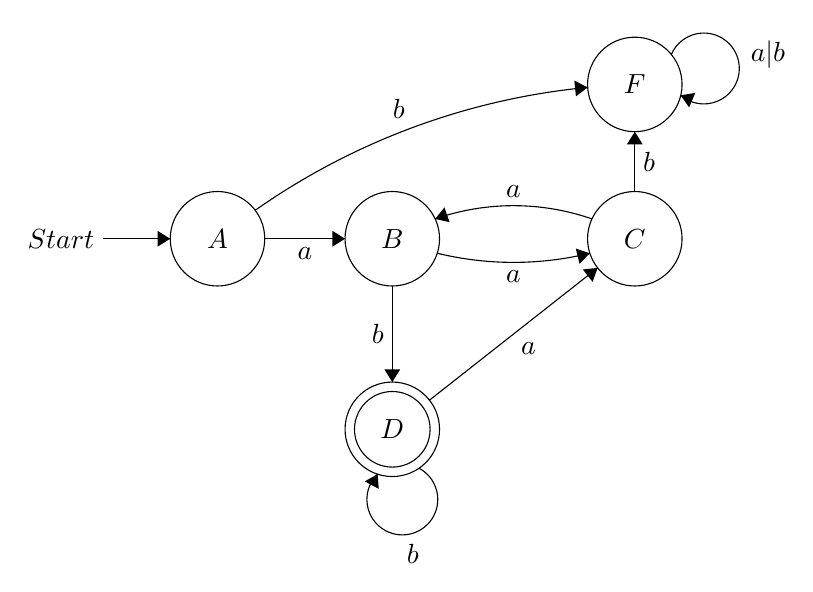
\begin{tikzpicture}[scale=0.2]
\tikzstyle{every node}+=[inner sep=0pt]
\draw [black] (14.1,-16.8) circle (3);
\draw (14.1,-16.8) node {$A$};
\draw [black] (25.2,-16.8) circle (3);
\draw (25.2,-16.8) node {$B$};
\draw [black] (40.6,-16.8) circle (3);
\draw (40.6,-16.8) node {$C$};
\draw [black] (25.2,-28.9) circle (3);
\draw (25.2,-28.9) node {$D$};
\draw [black] (25.2,-28.9) circle (2.4);
\draw [black] (40.6,-7) circle (3);
\draw (40.6,-7) node {$F$};
\draw [black] (6.8,-16.8) -- (11.1,-16.8);
\draw (6.3,-16.8) node [left] {$Start$};
\fill [black] (11.1,-16.8) -- (10.3,-16.3) -- (10.3,-17.3);
\draw [black] (17.1,-16.8) -- (22.2,-16.8);
\fill [black] (22.2,-16.8) -- (21.4,-16.3) -- (21.4,-17.3);
\draw (19.65,-17.3) node [below] {$a$};
\draw [black] (25.2,-19.8) -- (25.2,-25.9);
\fill [black] (25.2,-25.9) -- (25.7,-25.1) -- (24.7,-25.1);
\draw (24.7,-22.85) node [left] {$b$};
\draw [black] (26.888,-31.366) arc (62.1301:-225.8699:2.25);
\draw (26.5,-36.18) node [below] {$b$};
\fill [black] (24.27,-31.74) -- (23.45,-32.21) -- (24.34,-32.68);
\draw [black] (27.56,-27.05) -- (38.24,-18.65);
\fill [black] (38.24,-18.65) -- (37.3,-18.75) -- (37.92,-19.54);
\draw (33.85,-23.35) node [below] {$a$};
\draw [black] (37.747,-17.72) arc (-76.32345:-103.67655:20.501);
\fill [black] (37.75,-17.72) -- (36.85,-17.42) -- (37.09,-18.39);
\draw (32.9,-18.8) node [below] {$a$};
\draw [black] (16.494,-14.993) arc (125.10106:95.48887:44.042);
\fill [black] (37.61,-7.19) -- (36.76,-6.76) -- (36.86,-7.76);
\draw (25.61,-9.19) node [above] {$b$};
\draw [black] (40.6,-13.8) -- (40.6,-10);
\fill [black] (40.6,-10) -- (40.1,-10.8) -- (41.1,-10.8);
\draw (41.1,-11.9) node [right] {$b$};
\draw [black] (42.914,-5.109) arc (156.99462:-131.00538:2.25);
\draw (47.93,-5.08) node [right] {$a|b$};
\fill [black] (43.51,-7.69) -- (44.05,-8.46) -- (44.44,-7.54);
\draw [black] (27.918,-15.541) arc (109.18915:70.81085:15.158);
\fill [black] (27.92,-15.54) -- (28.84,-15.75) -- (28.51,-14.81);
\draw (32.9,-14.2) node [above] {$a$};
\end{tikzpicture}
\end{center}

	\end{solution}

\section{}
	Do the following pairs of regular expressions describe the same language?
	\subsection*{a)}
		$\epsilon|a(a|b)^{*}b$ and $(a(a|b)^{*}b)^{*}$
		\begin{solution}
		\end{solution}
		i) Let's call the former regular expression A (A = $\epsilon|a(a|b)^{*}b$) and the latter B (B =  $(a(a|b)^{*}b)^{*}$)\\~\\
		ii) Let's begin by observing that both regular expressions accept $\epsilon$. $\epsilon$ is a part of the definition of A but it is also allowed in B because of the kleene star. \\~\\
		iii) Now except for the empty string A has the only constraint that it accepts strings over the language $\{a,b\}$ which start with $a$ and end with $b$.\\~\\
		iv) Observe that the exact same constraints happen to apply to B if we leave out the outer kleene star: $a(a|b)^{*}b$. So assuming that the outer kleene star will have the value 1 ($a(a|b)^{*}b\{1\}$) the pairs do describe the same language. \\~\\
		v) If the outer kleene star has a value > 1 then we will still have a regular expression which accepts strings over the language \{a,b\} that start with a and end with b since that is a concatenation of the case where the kleene star has a value of 1. \\~\\
		vi) Any additional constraints that might exist when the kleene star has a value > 1 are therefore irrelevant since although the concatenation might not accept all strings over the language \{a,b\} that start with a and end with b all the strings it does accept do start with a and end with b and are therefore a subset of the special case when the outer kleene star has a value of 1.\\~\\
		From i - vi above we can see that both regular expression do in fact describe the same language which is: The empty string or a string that starts with a and ends with b.

	\subsection*{b)}
		$a^*$ and $(aaa)^{*}(a|aa)$
		\begin{solution}
		\end{solution}
		These regular expressions do not describe the same language since the former regular expression accepts $\epsilon$ but the latter does not.

\section{}
	Give a regular definition for the language consisting of all strings over the alphabet $\Sigma = \{a, b, c, d\}$ with no repeated letters.
	\begin{solution}
	\end{solution}
	Let's begin by defining some regular expression which will help with the final definition. \\
	$AInFront = a?b?c?d? | a?b?d?c? |a?c?b?d? | a?c?d?b? | a?d?b?c? | a?d?c?b?$\\
	$BInFront = b?a?c?d? | b?a?d?c? |b?c?a?d? | b?c?d?a? | b?d?a?c? | b?d?c?a?$\\
	$CInFront = c?b?a?d? | c?b?d?a? |c?a?b?d? | c?a?d?b? | c?d?b?a? | c?d?a?b?$\\
	$DInFront = d?b?c?a? | d?b?a?c? |d?c?b?a? | d?c?a?b? | d?a?b?c? | d?a?c?b?$\\
	With these definitions in place the final definition will be:\\
	$NoRepeat = AInFront | BInFront | CInFront | DInFront$

\end{document}